\begin{figure*}[t]
    \centering
    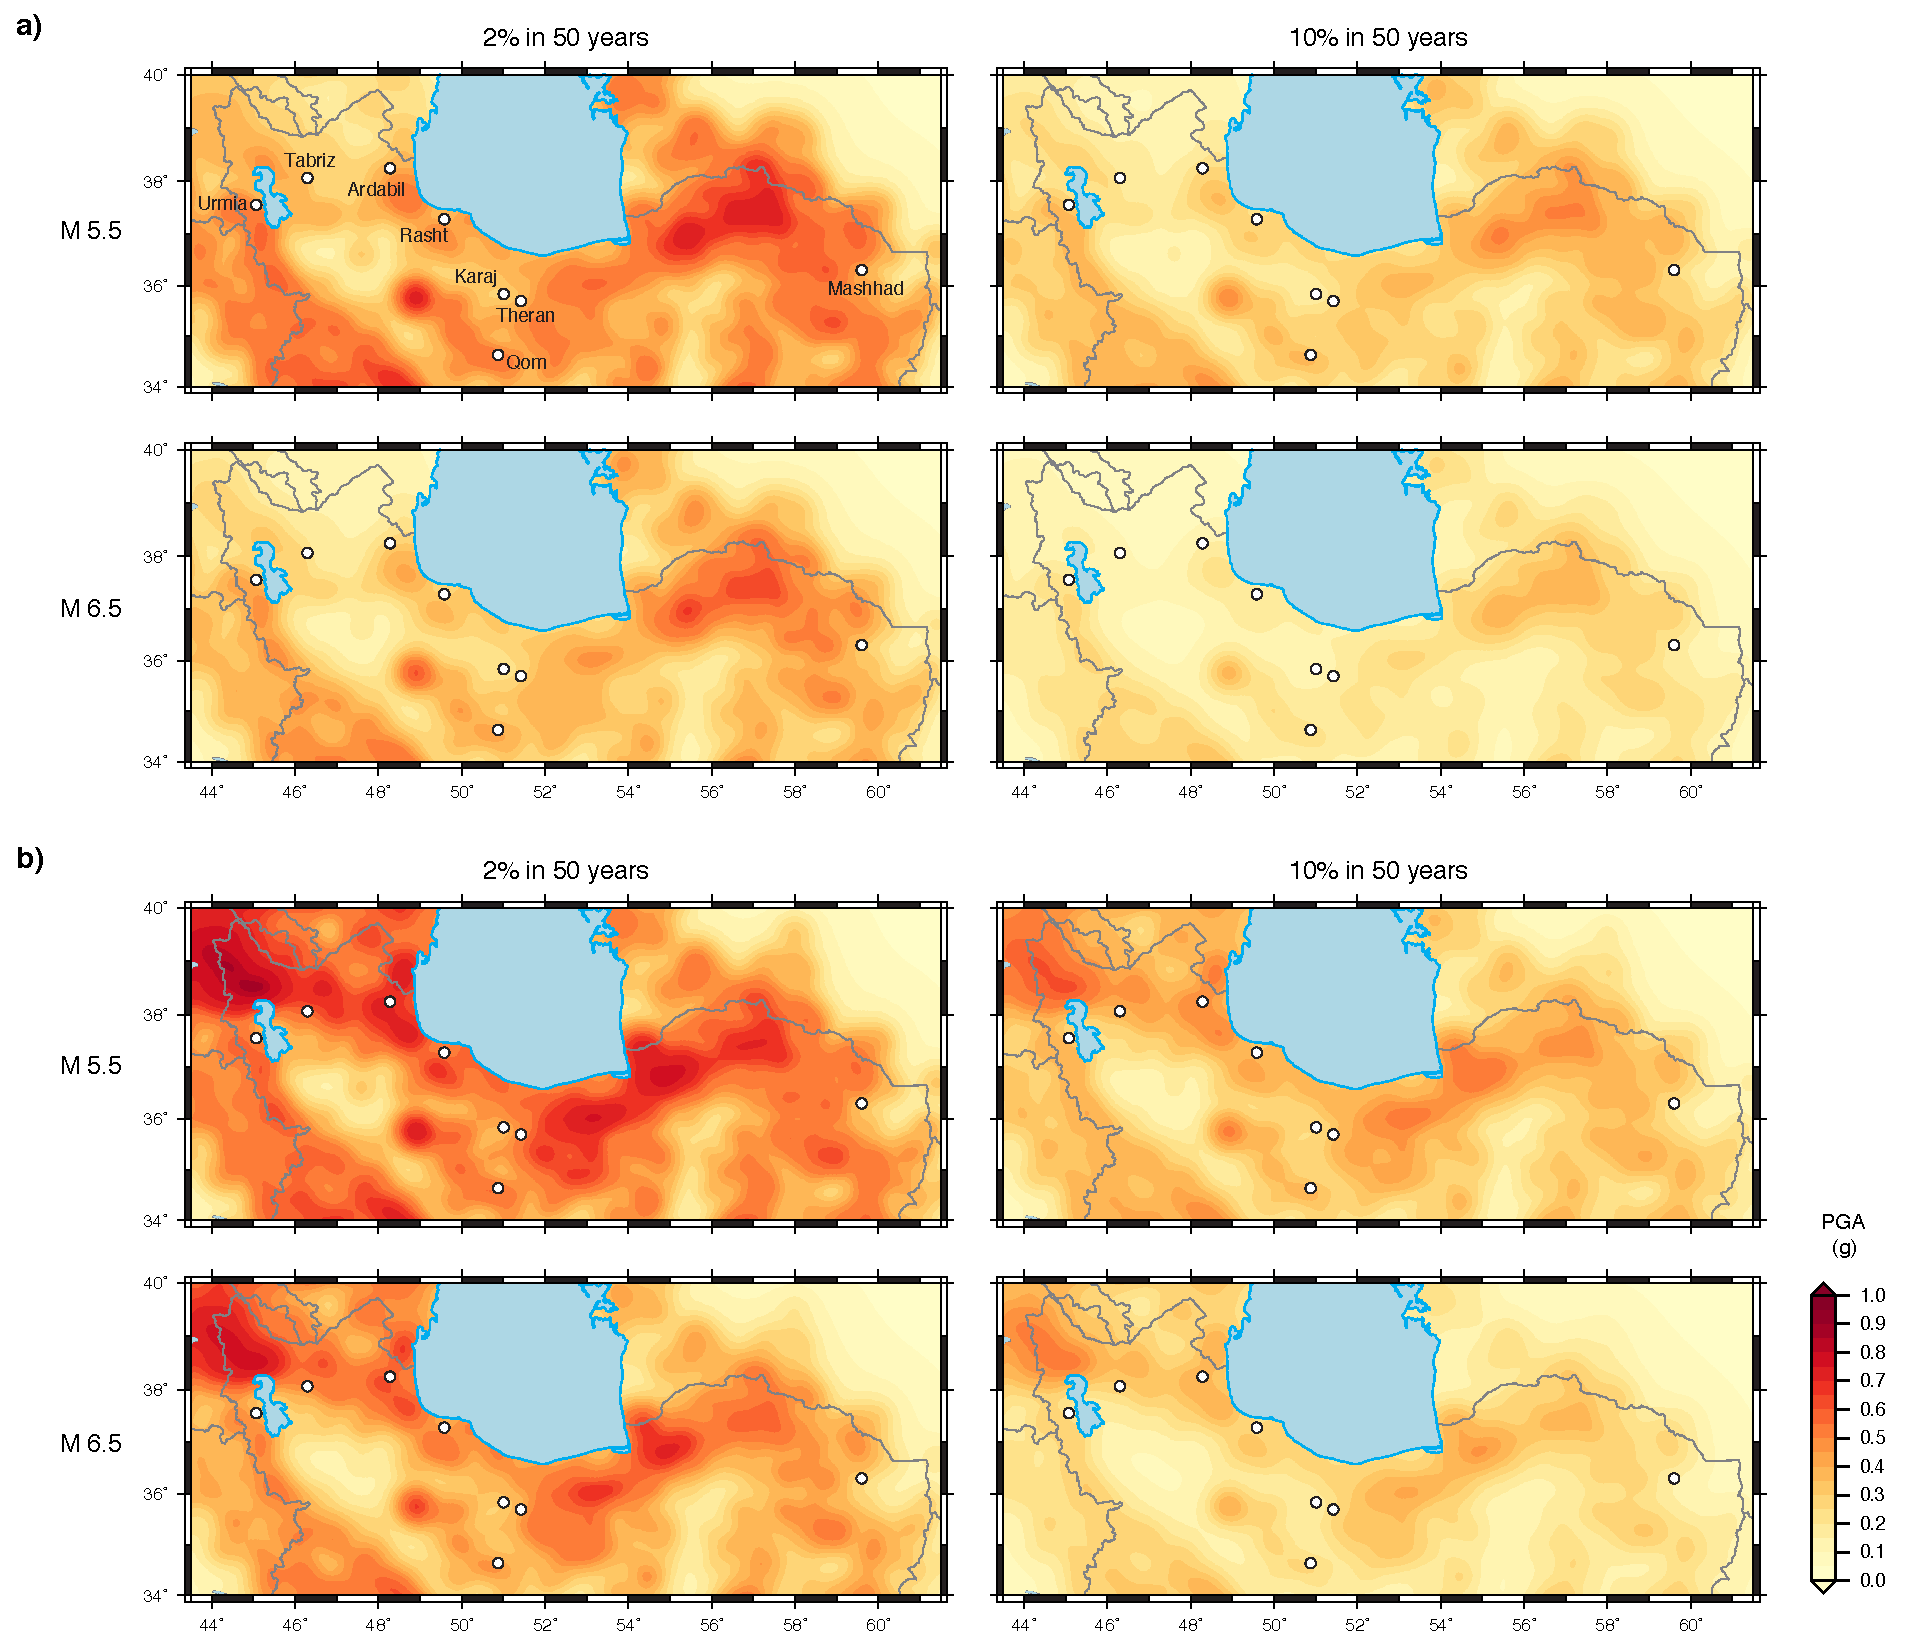
\includegraphics[width=\textwidth]{figures/pdf/figure-08.pdf} 
    \caption{Expected mean peak ground acceleration (PGA) for 2 and 10 percent of probability of exceedance in 50 years for (a) the five-seismic regions R model and (b) the uniform seismic region U model.}
    \label{fig:pga}
\end{figure*}

\begin{figure*}[t]
    \centering
    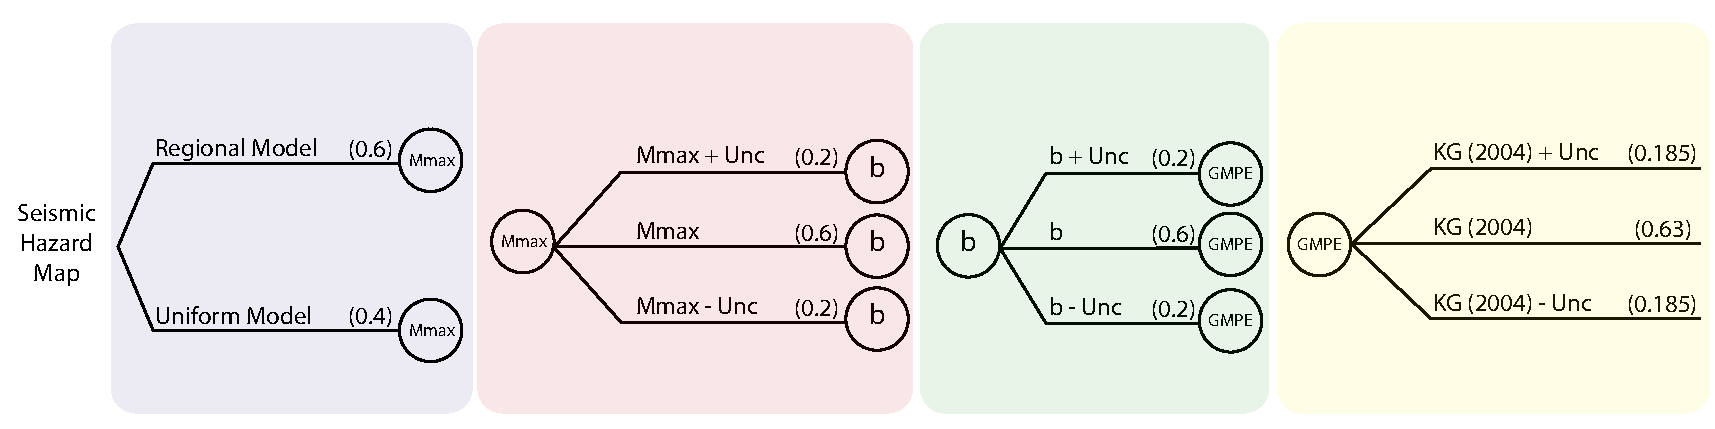
\includegraphics[width=\textwidth]{figures/pdf/figure-09.pdf} 
    \caption{Difference between the mean PGA values from models U and R for 2 (left) and 10 (right) percent probabilities of exceedance in 50 years.}
    \label{fig:pga.diff}
\end{figure*}

\begin{figure*}[t]
    \centering
    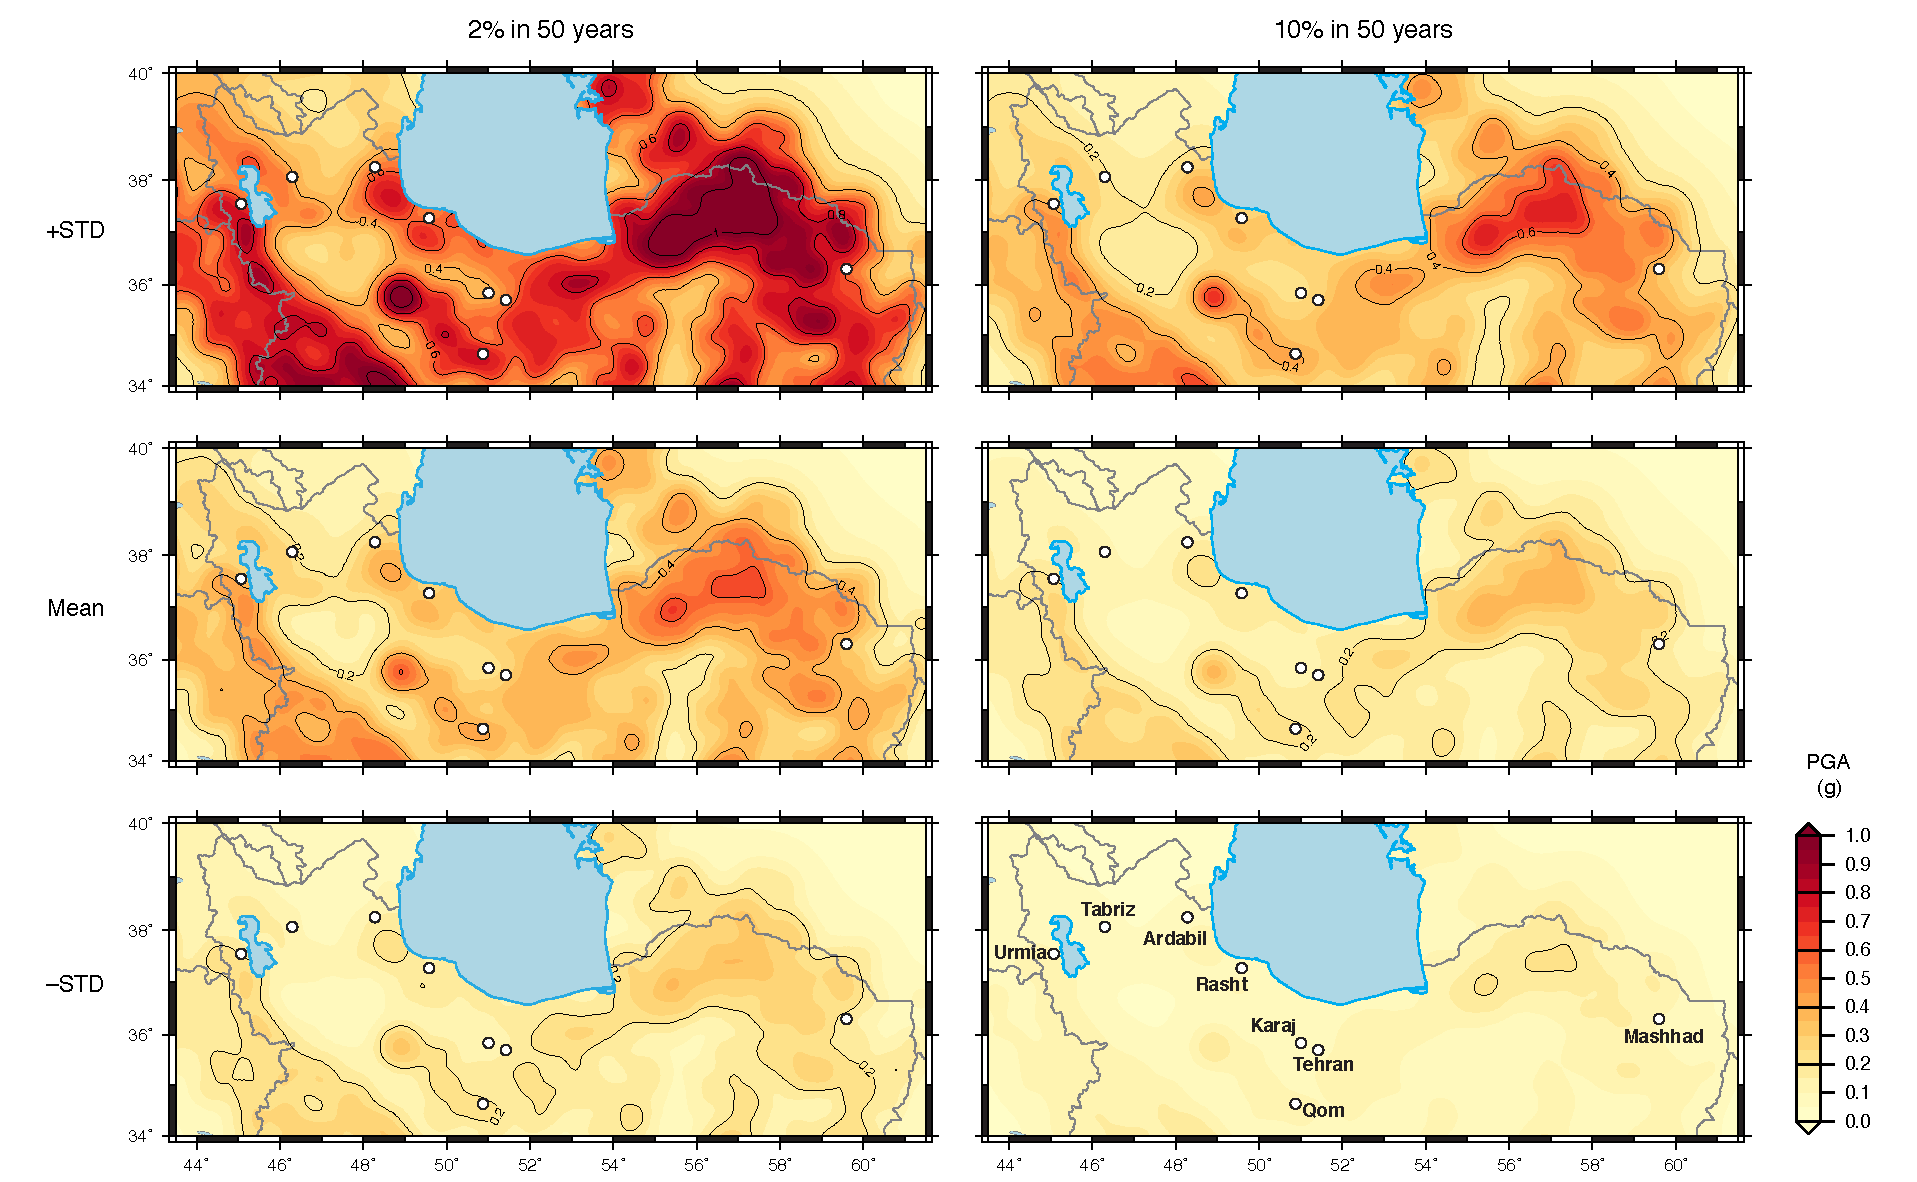
\includegraphics[width=\textwidth]{figures/pdf/figure-10.pdf} 
    \caption{Expected PGA values throughout the region of interest for 2 (left) and 10 (right) percent probability of exceeding an earthquake magnitude $M_w$ 5 using the combined model (R,U) hazard calculations. Mean expected values are shown in the middle, whereas the top and bottom frames correspond to the results obtained using plus and minus one standard deviation.}
    \label{fig:pga.ru.std}
\end{figure*}

\setlength{\tabcolsep}{1ex}

\begin{table*}[t]
\centering
\caption{Comparison of expected PGA values (in $g$) for selected cities in northern Iran between results obtained in this study and those of others previous studies. In our results, the values of the R and U models correspond to mean PGA values as shown also in Fig.~\ref{fig:pga}, and the (R,U) model values correspond to the combination of the R and U models shown in Fig.~\ref{fig:pga.ru.std}. The following codes are used for the references of other studies.
    Gh03: \citet{Ghodrati2003},
    Gh08: \citet{Ghodrati2008},
    Va11: \citet{Vafaie2011},
    Za12: \citet{Zare2012},
    Ab13: \citet{Abdi2013},
    BC14: \citet{BHRC2014},
    Go14: \citet{Golara2014},
    Az14: \citet{Abdollahzadeh2014a},
    Bo15: \citet{Boostan2015}.
    Kh16: \citet{Khodaverdian_2016_BSSA}
    }
\begin{tabular}{lccccccccc}
    \hline                                                                                                              \\[-1.6ex]
    \multicolumn{2}{l}{This study}
                     && \multicolumn{7}{c}{City (lat., lon.)}                                                           \\[0.6ex]
    \cline{4-10}                                                                                                        \\[-1.6ex]
            &        &&   Urmia     &   Tabriz    &   Ardabil   &   Rasht     &   Karaj     &   Tehran    &   Mashhad   \\
    Model   & Prob.  && (45.1,37.6) & (46.3,38.1) & (48.3,38.3) & (49.6,37.3) & (51.0,35.8) & (51.4,35.7) & (59.6,36.3) \\[0.6ex]
    \cline{1-2} \cline{4-10}                                                                                            \\[-1.6ex]
    R       &  10\%  &&   0.21      &   0.35      &   0.44      &   0.37      &   0.25      &   0.31      &   0.22      \\
            &   2\%  &&   0.35      &   0.60      &   0.73      &   0.61      &   0.41      &   0.53      &   0.39      \\
    U       &  10\%  &&   0.28      &   0.39      &   0.48      &   0.35      &   0.25      &   0.31      &   0.22      \\
            &   2\%  &&   0.50      &   0.67      &   0.76      &   0.58      &   0.42      &   0.53      &   0.38      \\
    (R,U)   &  10\%  &&   0.24      &   0.35      &   0.43      &   0.34      &   0.25      &   0.31      &   0.22      \\
            &   2\%  &&   0.38      &   0.61      &   0.73      &   0.58      &   0.40      &   0.53      &   0.39      \\
    \hline                                                                                                              \\[-1.6ex]
    \multicolumn{2}{l}{Other Studies}                                                                                   \\[0.6ex]
    \cline{1-2} \cline{4-10}                                                                                            \\[-1.6ex]
    Kh16    &  10\%  &&  0.15--0.20 & 0.15--0.20  & 0.30--0.35  & 0.15--0.20  & 0.15--0.20  & 0.15--0.20  & 0.10--0.15  \\
            &   2\%  &&  0.30--0.40 & 0.30--0.40  & 0.60--0.70  & 0.30--0.40  & 0.30--0.40  & 0.30--0.40  & 0.20--0.30  \\
    Bo15${}^{*}$
            &  10\%  &&   --        &   --        &   --        &   --        &   --        & 0.38--0.48  &   --        \\
    Az14    &  10\%  &&   --        &   --        &   --        & 0.25--0.30  &   --        &     --      &   --        \\
            &   2\%  &&   --        &   --        &   --        & 0.55--0.60  &   --        &     --      &   --        \\
    BC14    &  10\%  &&   0.30      &   0.35      &   0.30      &   0.30      &   0.35      &   0.35      &   0.30      \\
    Go14    &   2\%  && 0.30--0.50  & 0.90--1.20  & 0.50--0.70  & 0.50--0.70  & 0.70--0.90  & 0.70--0.90  & 0.70--0.90  \\
    Ab13${}^{*,\dagger}$
            &  10\%  &&   --        &   --        &   --        &   --        &   0.31      & 0.27--0.30  &   --        \\
            &   2\%  &&   --        &   --        &   --        &   --        &   0.42      &     --      &   --        \\
    Za12    &  10\%  && 0.35--0.50  & 0.35--0.50  & 0.35--0.50  & 0.50--0.65  & 0.35--0.50  & 0.35--0.50  & 0.35--0.50  \\
    Va11    &  10\%  &&   --        & 0.20--0.65  &   --        &   --        &   --        &     --      &     --      \\
            &   2\%  &&   --        & 0.30--0.90  &   --        &   --        &   --        &     --      &     --      \\
    Gh08    &  10\%  &&   --        &   --        &   --        &   0.10      &   --        &     --      &     --      \\
            &   2\%  &&   --        &   --        &   --        &   0.20      &   --        &     --      &     --      \\
    Gh03    &  10\%  &&   --        &   --        &   --        &   --        &   --        & 0.32--0.42  &     --      \\
    \hline                                                                                                              \\[-1.6ex]
    \multicolumn{10}{l}{\small{${}^{*}$ Used surface-wave magnitude $M_s$ 4.0 as magnitude threshold}}                  \\
    \multicolumn{10}{l}{\small{${}^{\dagger}$ Used $M_s$ 5.5 and 6.0 for Central-East and Alborz-Azerbaijan as magnitude threshold}}
\end{tabular}
\label{tab:pga}
\end{table*}


\section{Results and Analysis}

Using the data, parameters, and procedures just described, we considered two different hazard models based on whether we use the five distinct seismic hazard regions or the whole area of interest as a uniform seismic hazard region. We call these the R and U models, respectively. Using these models we obtained hazard curves and expected PGA values for two probabilities of exceedance, at 2 and 10 percent in 50 years for events exceeding magnitudes \myrevision{$M_w \geq 4.5$}. These probabilities correspond to return periods of 475 and 2475 years. For nomenclature purposes, we use the probabilities as a suffix on the model type. As an example, we refer to the results for 2 percent probability of exceedance in 50 years using the five-regions model as the R2, whereas for the case of 10 percent probability of exceedance when using the uniform model we use the tag name U10.

Our choice for the threshold magnitude is based on the assumption that at the local scale (where a point of interest is close to the source), the hazard will be controlled by events \myrevision{$M_w \geq 4.5$}, or conversely, \myrevision{$M_{min}$ was chosen based on the expected smallest magnitude capable of causing damage}. In turn, the 2 and 10 percent probability of exceedance in a \myrevision{50-year} span are considered a standard practice in seismic design, and are the probabilities used in the Iranian building code \citep{BHRC2014}.

In the R models, we computed the probability of exceedance of the ground motion separately for each region and then added their exceedance rates at a given level of ground motion in order to have the contribution of all regions for any given grid point within the region of interest. The results are obtained in the form of annual rate of exceedance. Expected PGA values are therefore a ``slice'' of the actual hazard curves cut across all grid points for a chosen exceedance rate.

Fig.~\ref{fig:pga} shows the expected mean PGA values obtained using the selected attenuation relationship in units of gravity (g) throughout the region of interest for the different models, R2, R10, U2 and U10. As can be expected, the highest PGA values are associated with the R2 and U2 models, and the lowest with the R10 and U10 models. For the R model results shown in Fig.~\ref{fig:pga}a, the highest levels of expected ground motion occur in the Kopeh Dagh region (near the border with Turkmenistan), and in a small area half-way between the city of Karaj and the Piranshahr fault, where a small concentration of events can be observed in Fig.~\ref{fig:catalog}b, as well as along the Piranshahr and Morvarid fault lines between the Zagros and Azerbaijan seismic regions (see Fig.~\ref{fig:selected}a for reference). The Azerbaijan seismic zone does not present equally high levels of expected ground motion. For the U model results shown in Fig.~\ref{fig:pga}b, on the other hand, the highest levels of expected ground motion are observed precisely in the area corresponding to the Azerbaijan seismic region, especially in the vicinity of the North Tabriz Fault system (see Fig.~\ref{fig:selected} for reference).

In general, the U models exhibit higher levels of expected ground motions when compared to their corresponding R models. This is illustrated in Fig.~\ref{fig:pga.diff}, which shows the difference between both models, U--R (U minus R). In this figure, positive values indicate that the U models have larger mean PGA values than the R models. As it can be seen, this is true practically throughout the whole region at very low levels, and in particular in the north-central region at a moderate level of up to 0.2 g and more predominantly in the north-western region of Azerbaijan at levels of about 0.2 to 0.45 g.

Overall, these results are consistent with the seismicity observed in Fig.~\ref{fig:catalog}. The R model results, however, seem to be more sensitive to the influence of large magnitude events observed in both the historical and modern seismicity maps, with \myrevision{a} concentration of strong earthquakes in the Alborz and Kopeh Dagh regions; whereas the U model results seem to be more sensitive to the influence of low-to-moderate magnitude events, especially in the Azerbaijan region. This is because of the higher $b$-value obtained for the Azerbaijan region in the R model as opposed to the lower value for the U model.

With this in mind, we make the following additional consideration. No one model (R or U) can be considered uniquely correct. Both carry a certain level of epistemic uncertainty. A means to address this is to use combinations of different models to incorporate information from all possible models. This would also be true, for instance, if in the future we were to consider other attenuation relationships. Here we also computed the expected levels of ground motion for a combination of the R and U models (with equal weights). We refer to this as the (R,U) model. The results of this combined model are shown in Fig.~\ref{fig:pga.ru.std} in the form of expected mean PGA values, along with the marginal values of plus and minus one standard deviation. Here, the standard deviation is carried forward in the calculation from the attenuation relationship and thus affects every grid point differently depending on the added contributions from each region. 

As it can be seen in Fig.~\ref{fig:pga.ru.std}, the combined (R,U) model follows more closely the distribution of the region's seismicity shown in Fig.~\ref{fig:catalog} as well as the major faults shown in Fig.~\ref{fig:selected}a, and thus we consider it to be a better assessment of the seismic hazard in the region. It displays well the contribution of the North Tabriz Fault system in the Azerbaijan region as well as the contribution of the Piranshahr and Morvarid faults in the Zagros region and that of the different faults in the Alborz and Kopeh Dagh regions. In Fig.~\ref{fig:pga.ru.std}, the highest PGAs are observed in the (R,U)2+STD model results, where the expected accelerations are of the order of 1.4 g to the northwest of \myrevision{the} city of Tabriz. These maximum values should, nonetheless, be interpreted with caution given the fact that predictions are based on rock-site assumptions and do not include any kind of site effects or other related conditions which may often contribute to mitigating peak accelerations.

\begin{figure*}[th!]
    \centering
    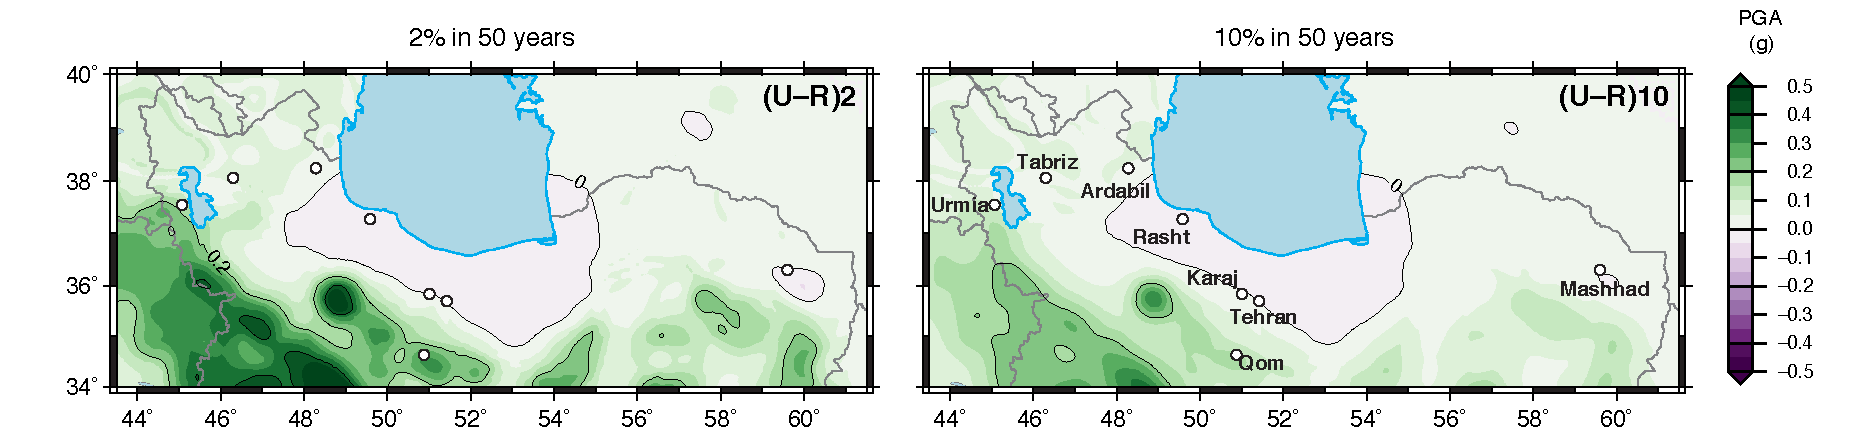
\includegraphics[width=\textwidth]{figures/pdf/figure-11} 
    \caption{Hazard curves representing the annual probability of exceedance as function of peak ground acceleration for six cities in northern Iran based on the two basic models considered in this study, R and U, and the combined model (R,U).}
    \label{fig:hazardcurve}
\end{figure*}

We also note that the overall distribution of mean PGA values shown in the middle panels in Fig.~\ref{fig:pga.ru.std} are the ones that best agree with the recent study by \citet{Khodaverdian_2016_BSSA}. These estimates also agree, on average, with other previous studies. For the north-west seismic regions of Azerbaijan and Zagros, for instance, \citet{Tavakoli1999} predicts maximum mean PGA (10\% in 50 years) values of 0.45 g near the North Tabriz Fault and the North Tehran Fault zones, where we find equivalent values to be between 0.35 and 0.50 g in the (R,U)10 model. Similarly, for the particular case of the city of Tabriz, \citet{Vafaie2011} obtained slightly higher expected accelerations on the order of 0.30--0.90 and 0.20--0.65 g for 2 and 10\% \myrevision{in 50 years}, respectively, where our mean values are about 0.53 and 0.36 g for the same corresponding probabilities. In the north-central region of Alborz, \citet{Ghodrati2003} and \citet{Boostan2015} predict PGA values of the order 0.27--0.46 g and 0.42--0.48 g for Tehran, where we found equivalent results to be about 0.25--0.35 g for a 10\% probability of exceedance \myrevision{in 50 years}. The latter estimate is in good agreement with \citet{Abdi2013}, who predicts PGA values in the vicinity of Karaj and Tehran to be on the order of 0.27--0.31 g for \myrevision{the same exceedance probability}. Results from \citet{Ghodrati2008} for the Gilan province around the city of Rasht are also on the same order of those shown in Fig.~\ref{fig:pga.ru.std}. Finally, for the city of Bojnurd in the northeast province of Khorasan in the Kopeh Dagh seismic region, \citet{Rahgozar2012} reports expected PGA values in the ranges of 0.28--0.49 and 0.15--0.22 g for 2 and 10\% \myrevision{in 50 years}, where we obtain mean values of 0.51 and 0.34 g, respectively.

Table \ref{tab:pga} shows a condensed version of these comparisons between our results and those of other previous studies for selected cities in northern Iran. As mentioned before, overall, our results are close \myrevision{to} or within the ranges from most studies. The only noticeable exceptions are the results of \citet{Golara2014}, whose expected PGA values are significantly higher than the rest, especially in the cities of Tabriz, Karaj, Tehran and Mashhad, where their results are closer to those of our upper (+STD) range of values. 

% ***

% Although not included here, we also computed expected PGA values for a magnitude threshold $M_w$ 4.5. In that case, our results are closer to those of \citet{Golara2014}, but deviate from the rest. In general, the smoothed seismicity method tends to lead to lower hazard estimations than those obtained using specific fault definitions (as opposed to point sources) where the concept of a threshold becomes unnecessary and the hazard, and thus is sensitive to the appropriate selection of the magnitude threshold.

% ***

Following the comparisons shown in Table \ref{tab:pga}, we looked into the more complete picture of the annual probabilities of exceedance as functions of PGA\myrevision{, also known as hazard curve}. The results are shown in Fig.~\ref{fig:hazardcurve} for six of the main cities in northern Iran considering the two basic R and U models and the combined (R,U) model. In each case we also show the range $\pm 1$ standard deviation (shaded areas). These hazard curves exemplify again the differences between the R and U models, which are more prominent in the northwest cities of Tabriz and Ardabil, where the U models yield higher expected values of PGA for any given annual probability of exceedance. Minor differences are also present in the results of the central cities of Karaj and Tehran, whereas for the cities of Urmia and Mashhad in the Zagros and Kopeh Dagh seismic zones, the R and U models yield similar if not equivalent hazard estimates. This is consistent with our previous observations regarding Figs.~\ref{fig:pga}, \ref{fig:pga.diff} and \ref{fig:pga.ru.std}.

\begin{figure}[t]
    \centering
    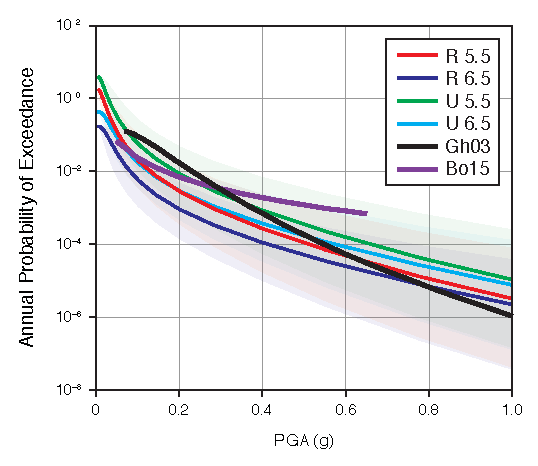
\includegraphics[width=0.48\textwidth]{figures/pdf/figure-12} 
    \caption{Hazard curve comparison between the models considered in this study and the results of two previous studies by \citet{Ghodrati2003} and \citet{Boostan2015} for the city of Tehran. Here, the two previous studies just mentioned are identified with the codes Gh03 and Bo15, respectively.}
    \label{fig:tehran}
\end{figure}

Last, we put additional attention on the results for the capital city of Tehran. We compare hazard curves obtained in this study against those computed by \citet{Ghodrati2003} and \citet{Boostan2015}. Our results are similar to those obtained by \citet{Ghodrati2003} in the range between 0.2 and 0.7 g (corresponding to annual probabilities of exceedance between $10^{-5}$ and $10^{-2}$), but the trend indicates we would obtain increasingly higher probabilities associated with PGA values above 0.8 g. Conversely, the trend in the hazard curve from \citet{Boostan2015} suggest the city is to expect significantly higher levels of ground motion at higher probability rates, which is contrary to our findings and those of \citet{Ghodrati2003}.
